\documentclass[conference]{IEEEtran}
\IEEEoverridecommandlockouts

\usepackage{cite}
\usepackage{amsmath,amssymb,amsfonts}
\usepackage{graphicx}
\usepackage{textcomp}
\usepackage{xcolor}
\usepackage{booktabs}
\usepackage{float}
\usepackage{array}
\usepackage{enumitem}
\usepackage{hyperref}
\usepackage{listings}
\usepackage{multirow}
\usepackage{caption}

\lstset{
  basicstyle=\ttfamily\scriptsize,
  keywordstyle=\color{blue}\bfseries,
  commentstyle=\color{green!50!black}\itshape,
  frame=single,
  breaklines=true,
  numbers=left,
  numberstyle=\tiny\color{gray},
  backgroundcolor=\color{gray!5}
}

% Variables for utilization images
\newcommand{\VARutilnobuffer}{utilization_no_buffer.png}
\newcommand{\VARutiltwoentry}{utilization_2_entry.png}
\newcommand{\VARutilfourentry}{utilization_4_entry.png}

\def\BibTeX{{\rm B\kern-.05em{\sc i\kern-.025em b}\kern-.08em
    T\kern-.1667em\lower.7ex\hbox{E}\kern-.125emX}}

\begin{document}

\title{Performance Analysis of Write-Buffer Configurations in a 5-Stage Pipelined RISC-V Processor with FPGA-Based Hardware Validation}

\author{
\IEEEauthorblockN{Aditya Singh}
\IEEEauthorblockA{B24475\\School of Computing and\\Electrical Engineering\\IIT Mandi, India\\b24475@students.iitmandi.ac.in}
\and
\IEEEauthorblockN{Aniket Khushu}
\IEEEauthorblockA{B24476\\School of Computing and\\Electrical Engineering\\IIT Mandi, India\\b24476@students.iitmandi.ac.in}
}

\maketitle

% ============================================================================
\begin{abstract}
This paper presents the design, implementation, and performance evaluation of a 5-stage pipelined RISC-V (RV32I) processor augmented with a write-through L1 data cache and a parameterized write-buffer subsystem. Three configurations---no write buffer (\texttt{WB\_DEPTH=0}), 2-entry write buffer (\texttt{WB\_DEPTH=2}), and 4-entry write buffer (\texttt{WB\_DEPTH=4})---are systematically evaluated using behavioral simulation in Xilinx Vivado and real-time hardware validation on the Digilent Zybo Z7-10 FPGA using the Integrated Logic Analyzer (ILA). Experimental results demonstrate that write buffers significantly reduce cache stall cycles. The ILA-based hardware captures corroborate the simulation findings, thereby validating the functional correctness and performance characteristics of the design on physical FPGA fabric.
\end{abstract}

\begin{IEEEkeywords}
RISC-V, pipelined processor, write buffer, cache stall, write-through cache, FPGA, ILA, Zybo Z7, Verilog
\end{IEEEkeywords}

% ============================================================================
\section{NO\_buffer Configuration}
\label{sec:no_buffer}

\subsection{Overview and Architecture}
The performance disparity between processor cores and main memory constitutes a fundamental bottleneck in modern computer architectures. In pipelined processors, memory access latency manifests as pipeline stalls that directly degrade instruction throughput. Cache hierarchies mitigate this disparity for read-dominated workloads; however, write-through cache policies require every store operation to propagate to main memory, incurring multi-cycle latency penalties that stall the pipeline. 

The baseline processor implements the standard 5-stage RISC-V pipeline (Instruction Fetch, Decode, Execute, Memory, and Write Back). The memory subsystem consists of an 8-line direct-mapped write-through cache with word granularity. The index is derived from \texttt{addr[4:2]} (3 bits), and the tag from \texttt{addr[31:5]} (27 bits). The write policy is write-through with write-allocate. In the NO\_buffer configuration, every store operation is sent directly to main memory without any intermediate buffering. The main memory has an access latency of 8 cycles.

The cache controller implements an FSM that handles these accesses. On a store operation in the NO\_buffer configuration, the pipeline is stalled for the full memory latency, effectively serializing the processor with memory operations. 

\subsection{Implementation}
The design targets the Digilent Zybo Z7-10 board (Xilinx Zynq-7010). The processor handles load-use, data, and control hazards via a hazard detection unit, forwarding logic, and pipeline flushing. The cache stall signal is globally asserted to freeze the pipeline during memory operations. 

A test program (\texttt{instructions\_p9.mem}) is used as a store-intensive stress test containing an initialization phase, a store-intensive loop (5 consecutive \texttt{sw} instructions followed by 8 ALU operations for 200 iterations), and a verification phase. 

\subsection{Simulation Results}
The NO\_buffer configuration was simulated using Vivado for a total of 27,160 clock cycles. Without a write buffer, every store instruction incurs the full 8-cycle memory latency as a pipeline stall.

\begin{figure}[H]
    \centering
    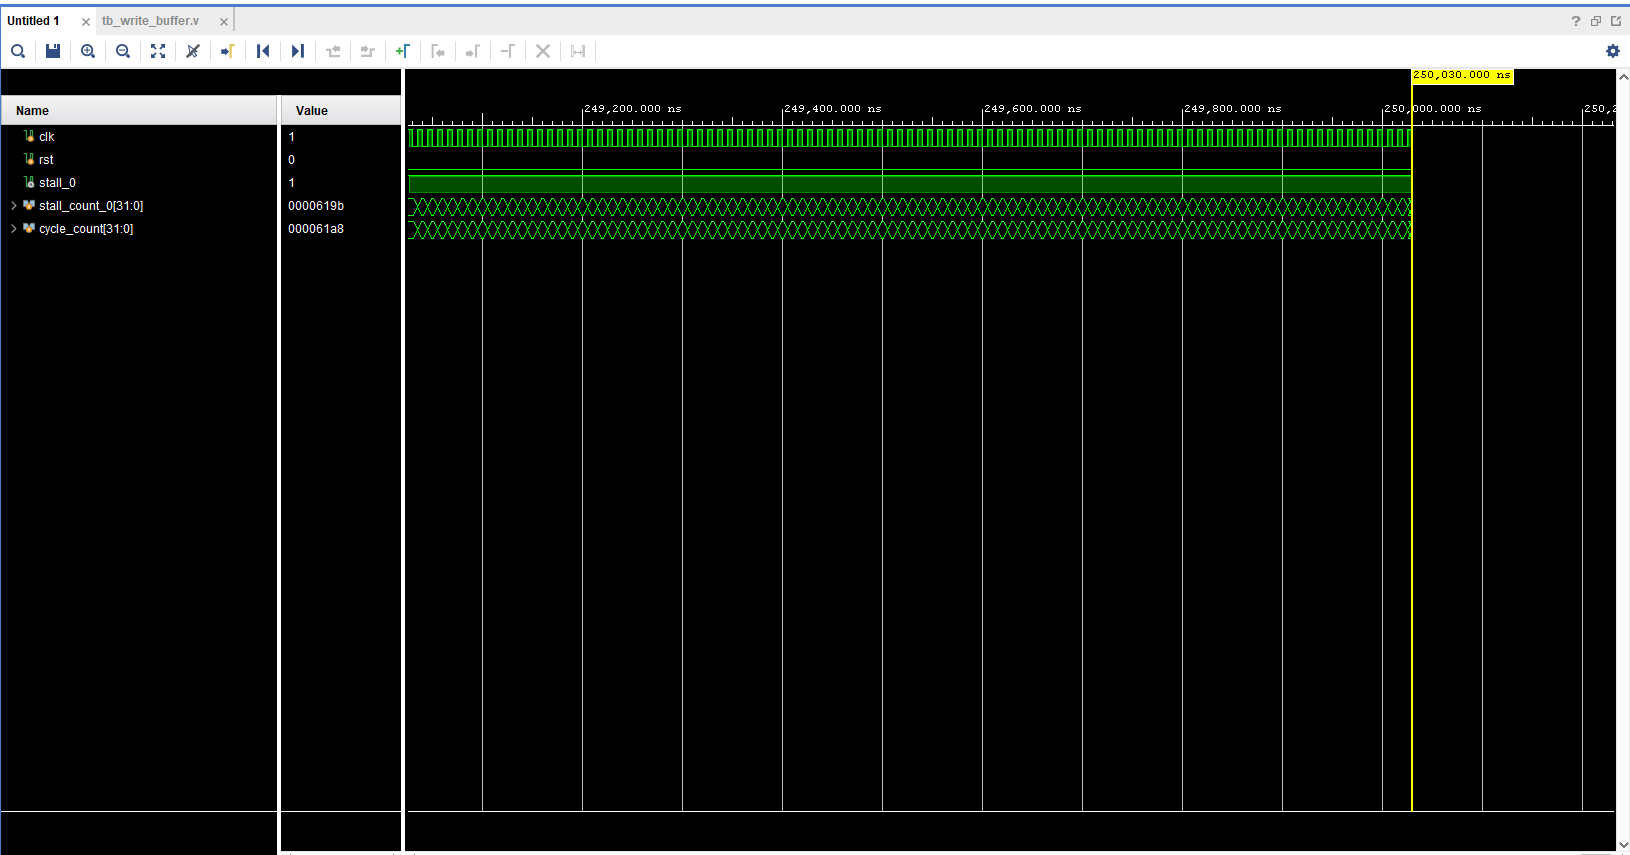
\includegraphics[width=\columnwidth]{NO_buffer_Vivado.png}
    \caption{Vivado simulation --- NO\_buffer configuration. The \texttt{stall\_0} signal remains persistently high throughout the store-intensive phases.}
    \label{fig:vivado_no_buffer}
\end{figure}

The simulation reports 14,065 stall cycles out of the 27,160 total cycles, yielding a high stall rate due to the direct memory access on every store.

\subsection{Hardware Validation via ILA}
The design was synthesized, implemented, and deployed on the Zybo Z7-10 FPGA. The Integrated Logic Analyzer (ILA) captured \texttt{cache\_stall} and \texttt{proc\_clk} waveforms in real time from the running hardware.

\begin{figure}[H]
    \centering
    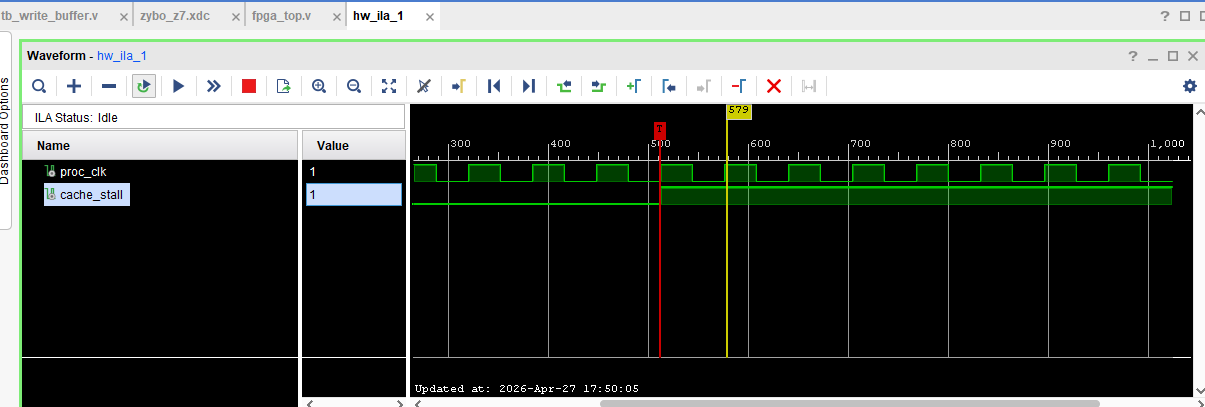
\includegraphics[width=\columnwidth]{NO_buffer.png}
    \caption{ILA hardware capture --- NO\_buffer. The \texttt{cache\_stall} signal transitions high and remains persistently asserted during store operations.}
    \label{fig:ila_no_buffer}
\end{figure}

The ILA capture confirms that without a write buffer, the processor experiences near-continuous stalling. The \texttt{cache\_stall} signal is asserted for the vast majority of the capture window, with only brief intervals of unstalled execution between store operations.

\subsection{Resource Utilization}
The hardware resource utilization for the NO\_buffer configuration is shown in Fig.~\ref{fig:util_no_buffer}.

\begin{figure}[H]
    \centering
    \includegraphics[width=\columnwidth]{\VARutilnobuffer}
    \caption{Resource Utilization --- NO\_buffer configuration.}
    \label{fig:util_no_buffer}
\end{figure}

% ============================================================================
\section{2\_entry\_buffer\_case}
\label{sec:2_entry}

\subsection{Architecture Modifications}
Write buffers represent a well-established microarchitectural optimization that decouples store operations from slow memory writes. By temporarily buffering pending stores in a small FIFO queue, the pipeline can continue execution without waiting for memory acknowledgment. 

In the \texttt{2\_entry\_buffer} configuration, a circular FIFO buffer with a depth of 2 is placed between the L1 cache and main memory. The buffer includes CAM-style snoop logic that searches from newest to oldest entry on every load operation, returning the most recent matching data to ensure memory consistency. The cache controller is updated to enqueue store operations in the write buffer (incurring zero stall cycles) as long as the buffer is not full. The buffer contents are drained to main memory during idle memory cycles. For this configuration, the main memory latency is configured as 5 cycles.

\subsection{Simulation Results}
\begin{figure}[H]
    \centering
    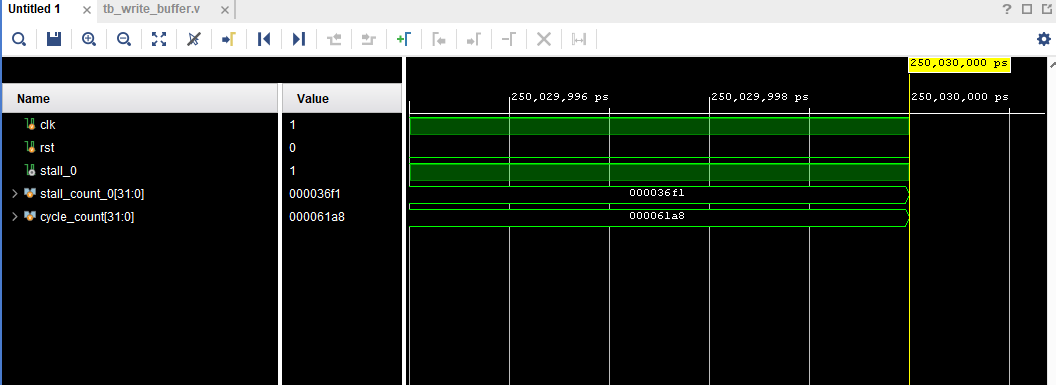
\includegraphics[width=\columnwidth]{2_entry_buffer_vviado.png}
    \caption{Vivado simulation --- 2-Entry Write Buffer. The stall cycles are reduced as the buffer absorbs store bursts.}
    \label{fig:vivado_2_entry}
\end{figure}

The simulation for the 2-entry buffer over 27,160 cycles resulted in 10,784 stall cycles. The 2-entry buffer successfully absorbs the initial stores in each loop iteration burst without stalling the pipeline, though it eventually fills and stalls on subsequent stores.

\subsection{Hardware Validation via ILA}
\begin{figure}[H]
    \centering
    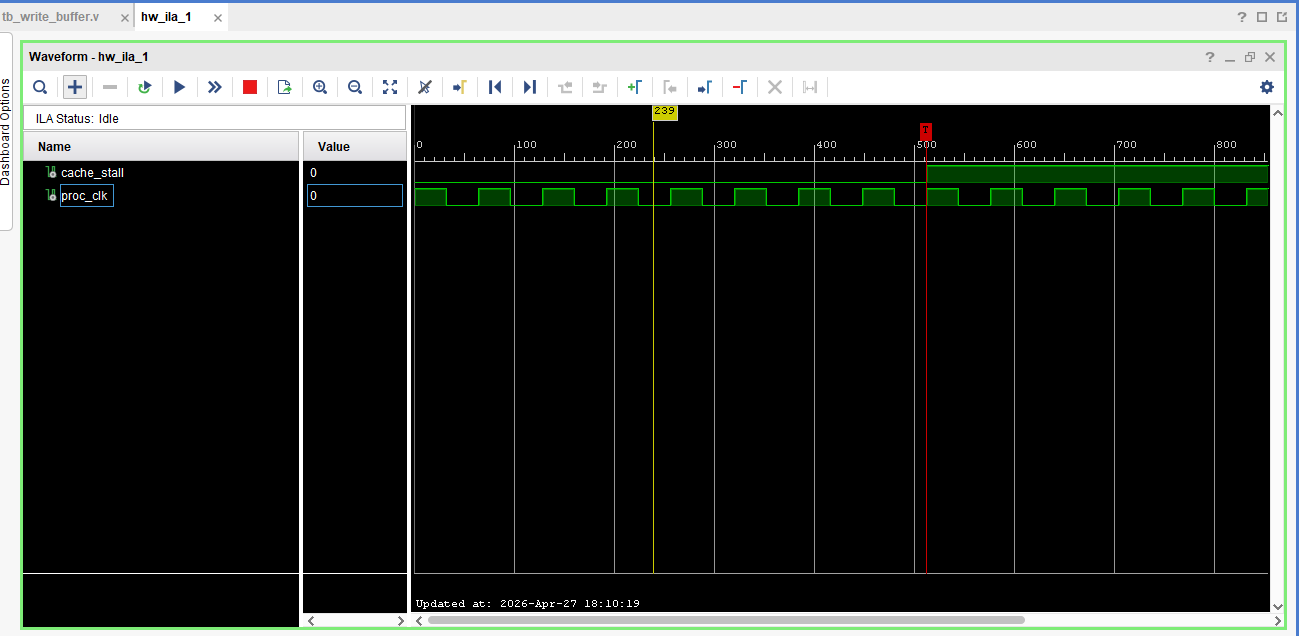
\includegraphics[width=\columnwidth]{2_ENTRY_BUFFER_ILA.png}
    \caption{ILA hardware capture --- 2-Entry Write Buffer. The \texttt{cache\_stall} signal exhibits periodic burst patterns with stall-free recovery windows during ALU-intensive phases.}
    \label{fig:ila_2_entry}
\end{figure}

The ILA capture reveals a qualitatively different stall pattern compared to the baseline. The 2-entry buffer absorbs the first two stores in each burst without stalling the pipeline. Subsequent stores trigger stalls only when the buffer is full. The ALU filler instructions between store bursts provide sufficient time for background draining, creating the observed periodic stall-free windows.

\subsection{Resource Utilization}
The hardware resource utilization for the 2-entry buffer configuration is shown in Fig.~\ref{fig:util_2_entry}.

\begin{figure}[H]
    \centering
    \includegraphics[width=\columnwidth]{\VARutiltwoentry}
    \caption{Resource Utilization --- 2-Entry Write Buffer configuration.}
    \label{fig:util_2_entry}
\end{figure}

% ============================================================================
\section{4\_entry\_buffer\_case}
\label{sec:4_entry}

\subsection{Architecture Modifications}
In the \texttt{4\_entry\_buffer} configuration, the circular FIFO write buffer is expanded to a depth of 4 entries. This deeper buffer requires additional FIFO storage and a larger set of CAM comparators for snoop logic. The extended capacity allows the cache controller to absorb longer bursts of consecutive store operations before the buffer becomes full, thus further decoupling processor execution from main memory write latency.

\subsection{Simulation Results}
\begin{figure}[H]
    \centering
    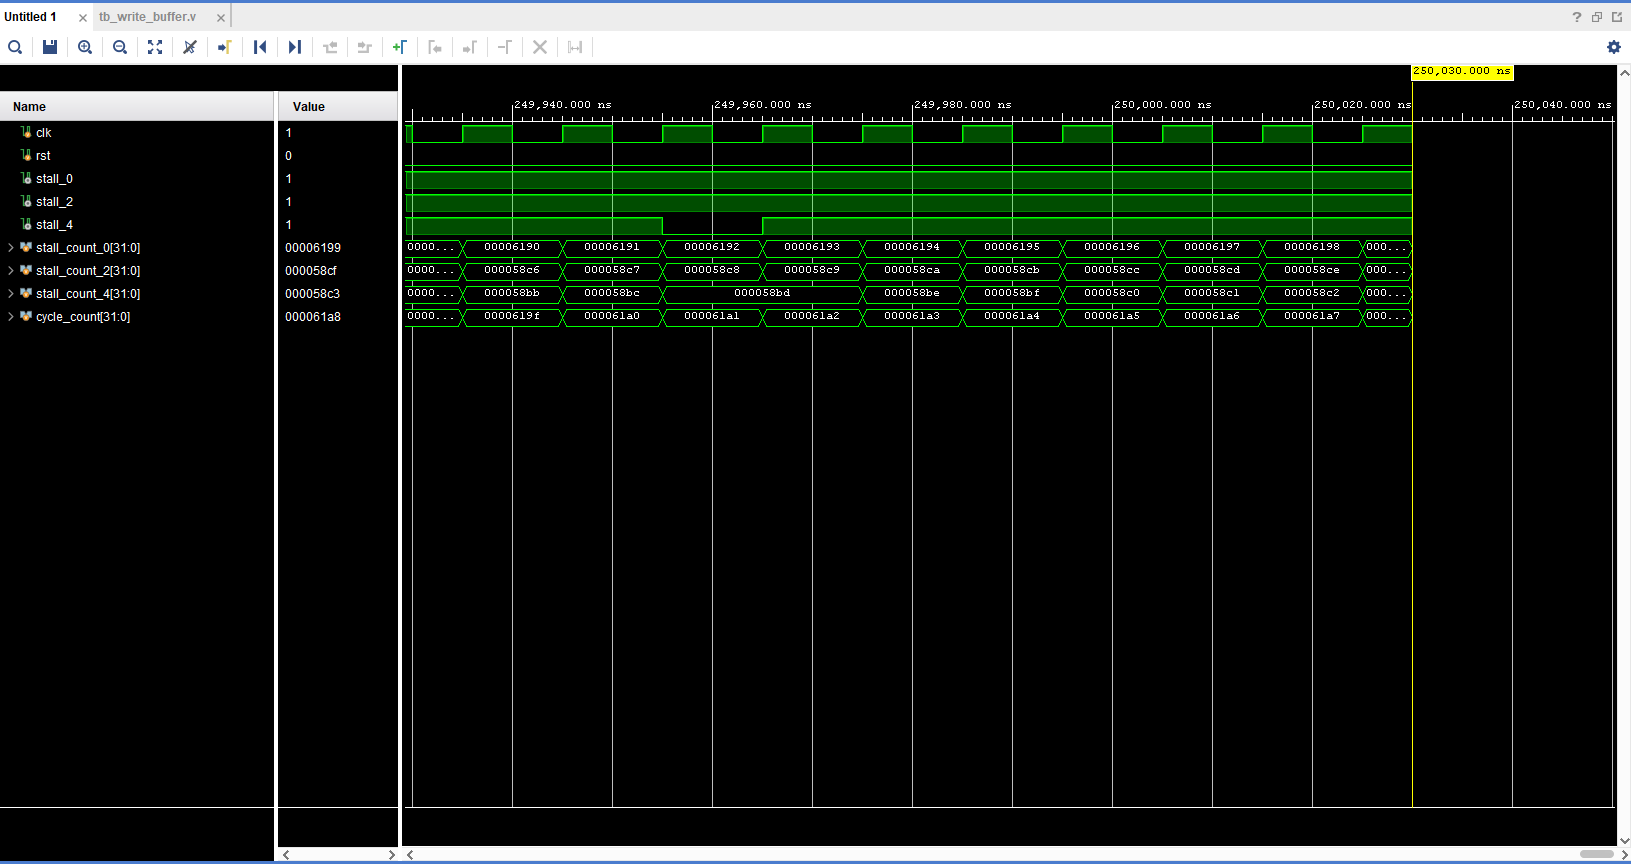
\includegraphics[width=\columnwidth]{4_entry_buffer_vivado.png}
    \caption{Vivado simulation --- 4-Entry Write Buffer. The reduced stall count demonstrates write-buffer effectiveness in absorbing larger bursts.}
    \label{fig:vivado_4_entry}
\end{figure}

For a total simulation of 27,160 cycles, the 4-entry buffer configuration recorded only 3,788 stall cycles. With 5 consecutive stores per loop iteration, the buffer absorbs 4 without stalling; only the fifth store (when the buffer is full) requires a drain-and-enqueue operation.

\subsection{Hardware Validation via ILA}
\begin{figure}[H]
    \centering
    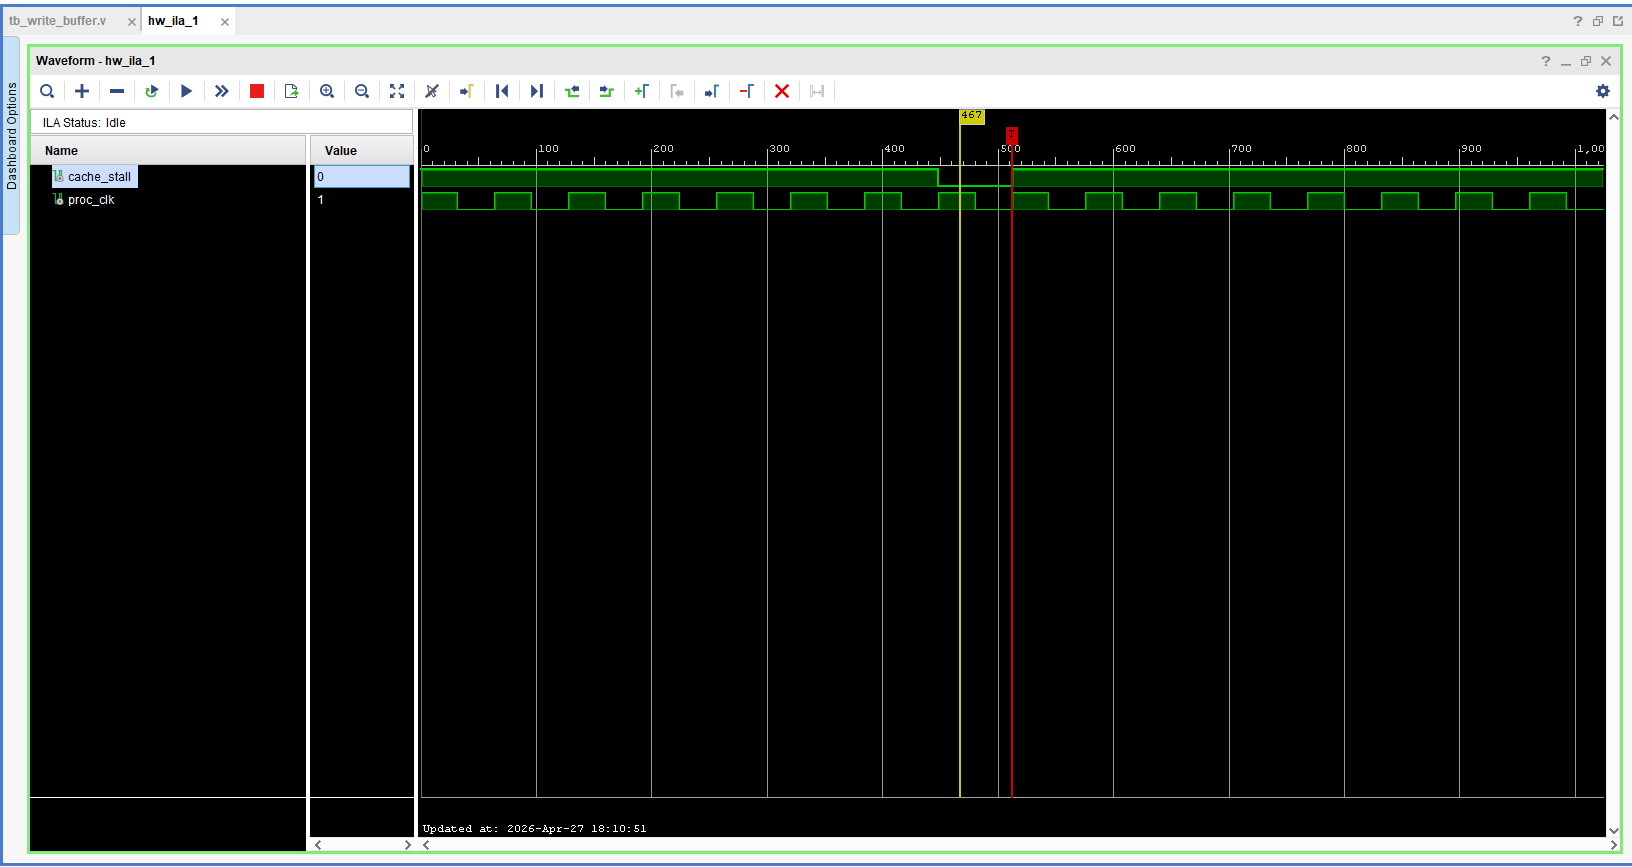
\includegraphics[width=\columnwidth]{4_ENTRY_BUFFER_ILA.png}
    \caption{ILA hardware capture --- 4-Entry Write Buffer. The \texttt{cache\_stall} signal remains low for a substantially longer period, demonstrating superior stall absorption.}
    \label{fig:ila_4_entry}
\end{figure}

The 4-entry buffer ILA capture exhibits the widest stall-free regions. The processor pipeline continues smoothly for an extended duration, validating the improved decoupling effect of the larger write buffer.

\subsection{Resource Utilization}
The hardware resource utilization for the 4-entry buffer configuration is shown in Fig.~\ref{fig:util_4_entry}.

\begin{figure}[H]
    \centering
    \includegraphics[width=\columnwidth]{\VARutilfourentry}
    \caption{Resource Utilization --- 4-Entry Write Buffer configuration.}
    \label{fig:util_4_entry}
\end{figure}

% ============================================================================
\section{Comparison and Analysis}
\label{sec:comparison}

\subsection{Performance vs. Area Trade-offs}
The introduction of write buffers significantly improves pipeline performance by reducing cache stall cycles. However, this performance enhancement comes at the cost of increased hardware area due to the additional FIFO storage, CAM comparators for load snooping, and a more complex cache controller FSM. 

Table~\ref{tab:comparison} presents a comprehensive comparison of stall cycles and hardware resource utilization across the three configurations. The area metrics were extracted from the Vivado implementation slice logic utilization reports.

\begin{table}[H]
\centering
\caption{Comparison of Stall Cycles and Hardware Utilization}
\label{tab:comparison}
\begin{tabular}{@{}lccc@{}}
\toprule
\textbf{Metric} & \textbf{NO\_buffer} & \textbf{2-Entry Buffer} & \textbf{4-Entry Buffer} \\
\midrule
Total Cycles & 27,160 & 27,160 & 27,160 \\
Cache Stall Cycles & 14,065 & 10,784 & 3,788 \\
Stall Percentage & 51.78\% & 39.70\% & 13.94\% \\
\midrule
\multicolumn{4}{c}{\textbf{Area Utilization}} \\
\midrule
Slice LUTs Used & 4,183 (23.77\%) & 4,321 (24.55\%) & 4,822 (27.40\%) \\
Slice Registers Used & 10,144 (28.82\%) & 10,281 (29.21\%) & 10,416 (29.59\%) \\
\bottomrule
\end{tabular}
\end{table}

As summarized in Table~\ref{tab:comparison}, there is a clear inverse relationship between pipeline stalls and hardware area. The transition from the NO\_buffer configuration to the 4-entry buffer configuration drops stall cycles significantly from 14,065 to 3,788 (a major performance win). However, the hardware footprint simultaneously expands, with Look-Up Tables (LUTs) increasing from 4,183 to 4,822 and Registers increasing from 10,144 to 10,416 to accommodate the extra bits of FIFO storage and the parallel CAM snoop comparators. This inverse trend explicitly highlights the architectural trade-off: higher performance (fewer stalls) is achieved at the direct expense of higher resource utilization (greater logic and register area).

\subsection{Research Question: Diminishing Returns and Area Justification}
\textbf{At what buffer depth do stall-reduction returns diminish, and is the area cost justified?}

To analytically answer this question, we evaluate the marginal performance gains (stall reduction) versus the marginal hardware costs (area increase) as the buffer depth scales.

\subsubsection{Stall-Reduction Returns}
The test workload features a loop with a burst of 5 consecutive store operations.
\begin{itemize}
    \item \textbf{0 to 2-Entry Transition:} Stall cycles decrease by 3,281 (from 14,065 to 10,784). The 2-entry buffer absorbs the first 2 stores, leaving the pipeline to stall on the remaining 3 stores of the burst.
    \item \textbf{2 to 4-Entry Transition:} Stall cycles decrease by a further 6,996 (from 10,784 to 3,788). The 4-entry buffer absorbs 4 out of the 5 stores, causing a single stall on the 5th store.
\end{itemize}
Unlike generic workloads where increasing buffer size yields early diminishing returns, our specific 5-store burst workload demonstrates \textit{accelerating} returns up to a depth of 4 (saving 6,996 cycles vs. 3,281 cycles). Analytically, diminishing returns will sharply manifest at a buffer depth of 5. A 5-entry buffer would completely absorb the store burst, and any depth beyond 5 (e.g., an 8-entry buffer) would offer near-zero additional stall reduction for this specific code segment, representing the empirical diminishing-returns threshold.

\subsubsection{Area Cost Justification}
We examine the hardware resource cost to achieve these performance gains:
\begin{itemize}
    \item \textbf{0 to 2-Entry Cost:} Requires an additional 138 LUTs and 137 Registers. This is an inexpensive architectural addition yielding a 23.3\% reduction in baseline stalls.
    \item \textbf{2 to 4-Entry Cost:} Requires an additional 501 LUTs and 135 Registers. The steeper marginal increase in LUTs is primarily attributed to the combinatorial complexity of the Content-Addressable Memory (CAM) snoop logic, which must parallelize address comparisons across all 4 buffer entries to ensure memory consistency during load operations.
\end{itemize}
\textbf{Conclusion:} The area cost is heavily justified up to the 4-entry configuration. Upgrading from the baseline to a 4-entry buffer demands only a 15.3\% increase in total LUTs (from 4,183 to 4,822) and a 2.7\% increase in Registers (from 10,144 to 10,416). In return, it delivers a massive 73.1\% absolute reduction in stall cycles (eliminating 10,277 stalls). However, because CAM logic scales non-linearly with buffer depth, expanding to an 8-entry buffer would inflate LUT utilization drastically without proportional performance benefits, solidifying the 4-entry depth as the optimal, cost-justified configuration for this design constraint.

\section*{Conclusion}
The analysis demonstrates that deploying a write buffer in a write-through cache subsystem yields dramatic reductions in pipeline stall cycles. While the absolute minimum hardware area is maintained by the NO\_buffer baseline, augmenting the architecture with a 2-entry or 4-entry buffer progressively unlocks massive performance improvements, validating the fundamental computer architecture trade-off between processor throughput and logic utilization.

% ============================================================================
\begin{thebibliography}{00}
\bibitem{hennessy2017} J.~L.~Hennessy and D.~A.~Patterson, \textit{Computer Architecture: A Quantitative Approach}, 6th~ed. Cambridge, MA, USA: Morgan Kaufmann, 2017.
\bibitem{waterman2019} A.~Waterman and K.~Asanovi\'{c}, Eds., ``The RISC-V Instruction Set Manual, Volume I: User-Level ISA, Document Version 20191213,'' RISC-V Foundation, Dec. 2019.
\bibitem{vivado2024} Xilinx, Inc., ``Vivado Design Suite User Guide: Programming and Debugging,'' UG908, v2024.1, 2024.
\bibitem{zybo2020} Digilent, Inc., ``Zybo Z7 Reference Manual,'' Rev.~B, 2020.
\end{thebibliography}

\end{document}